% 1977 年江苏南通卷第十题：两根钢绳悬吊货物的受力示意（按源卷第 5 页布局）：
% 结点处 F1（左上）、F2（右上）两条拉力与竖直向下重力 P，上方虚线把 F1、F2
% 作用线延长到竖直线交成力三角形，1、2 号角在结点处，3 号角在顶点处，4 号角在 F1 箭头端处
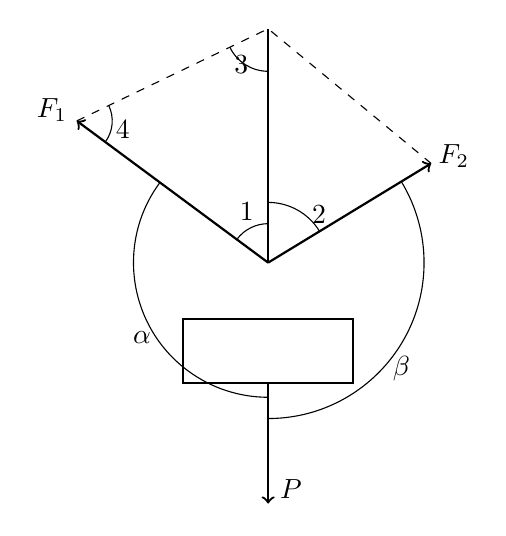
\begin{tikzpicture}[scale=0.9]
  \coordinate (K) at (0,0);
  \coordinate (T) at (0,3.3);
  \coordinate (L) at (-2.7,2.0);
  \coordinate (R) at (2.3,1.4);
  \draw[thick,->] (0,0)--(L);
  \node at (-3.05,2.15) {$F_1$};
  \draw[thick,->] (0,0)--(R);
  \node at (2.62,1.5) {$F_2$};
  \draw[thick] (0,0)--(T);
  \draw[dashed] (L)--(T);
  \draw[dashed] (R)--(T);
  \draw[thick] (-1.2,-0.8) rectangle (1.2,-1.7);
  \draw[thick,->] (0,-1.7)--(0,-3.4);
  \node at (0.32,-3.2) {$P$};
  \draw (90:0.55) arc[start angle=90, end angle=143.5, radius=0.55];
  \node at (-0.3,0.72) {$1$};
  \draw (90:0.85) arc[start angle=90, end angle=31.3, radius=0.85];
  \node at (0.72,0.68) {$2$};
  \begin{scope}[shift={(0,3.3)}]
    \draw (205.7:0.6) arc[start angle=205.7, end angle=270, radius=0.6];
  \end{scope}
  \node at (-0.38,2.8) {$3$};
  \begin{scope}[shift={(-2.7,2.0)}]
    \draw (25.7:0.5) arc[start angle=25.7, end angle=-36.5, radius=0.5];
  \end{scope}
  \node at (-2.05,1.88) {$4$};
  \draw (143.5:1.9) arc[start angle=143.5, end angle=270, radius=1.9];
  \node at (-1.78,-1.05) {$\alpha$};
  \draw (270:2.2) arc[start angle=270, end angle=391.3, radius=2.2];
  \node at (1.88,-1.5) {$\beta$};
\end{tikzpicture}
